\sectionthree{Space subdivision problems}
\begin{python0}
from solutions import *; clear() 
\end{python0}

What is the maximum number of regions do you get when you
cut up a 2-dimensional space by $n$ lines.
With one line:
\begin{center}
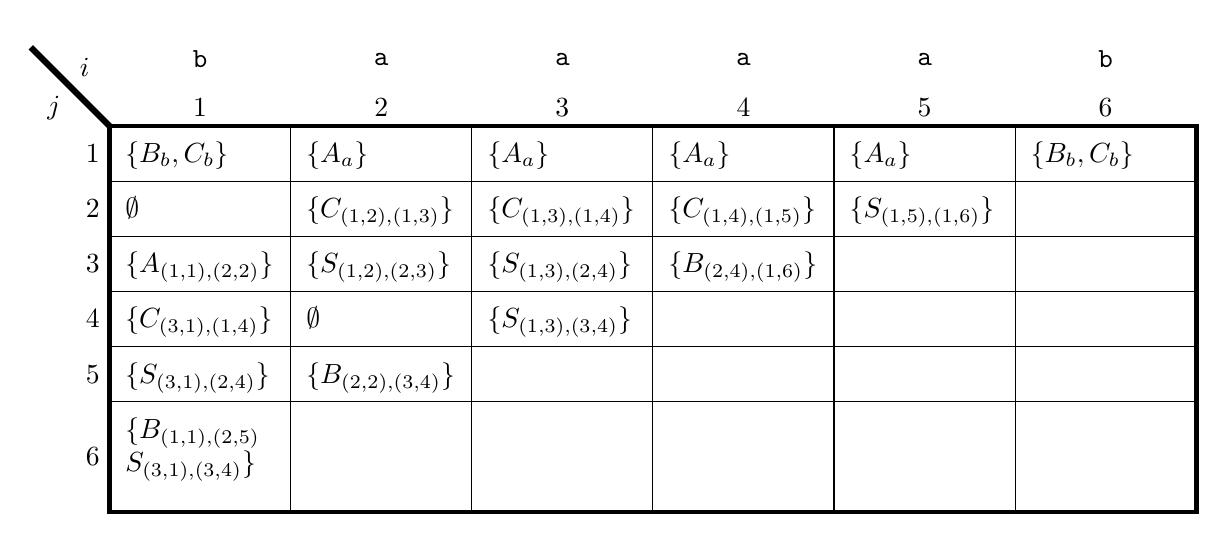
\begin{tikzpicture}

\draw (1.15, -0.35)
  node[draw, , , color=black,
       rounded corners=0cm, inner sep=0.2cm] {

\begin{minipage}[t][0.3cm]{1.9cm}
\mbox{}

\end{minipage}

};
\draw (1.15, -0.35) node[color=black,
 inner sep=0.2cm] {
 
\begin{minipage}[t][0.3cm]{1.9cm}
$\{B_b,C_b\}$
\end{minipage}

};
\draw (3.4499999999999997, -0.35)
  node[draw, , , color=black,
       rounded corners=0cm, inner sep=0.2cm] {

\begin{minipage}[t][0.3cm]{1.9cm}
\mbox{}

\end{minipage}

};
\draw (3.4499999999999997, -0.35) node[color=black,
 inner sep=0.2cm] {
 
\begin{minipage}[t][0.3cm]{1.9cm}
$\{A_a\}$
\end{minipage}

};
\draw (5.75, -0.35)
  node[draw, , , color=black,
       rounded corners=0cm, inner sep=0.2cm] {

\begin{minipage}[t][0.3cm]{1.9cm}
\mbox{}

\end{minipage}

};
\draw (5.75, -0.35) node[color=black,
 inner sep=0.2cm] {
 
\begin{minipage}[t][0.3cm]{1.9cm}
$\{A_a\}$
\end{minipage}

};
\draw (8.049999999999999, -0.35)
  node[draw, , , color=black,
       rounded corners=0cm, inner sep=0.2cm] {

\begin{minipage}[t][0.3cm]{1.9cm}
\mbox{}

\end{minipage}

};
\draw (8.049999999999999, -0.35) node[color=black,
 inner sep=0.2cm] {
 
\begin{minipage}[t][0.3cm]{1.9cm}
$\{A_a\}$
\end{minipage}

};
\draw (10.35, -0.35)
  node[draw, , , color=black,
       rounded corners=0cm, inner sep=0.2cm] {

\begin{minipage}[t][0.3cm]{1.9cm}
\mbox{}

\end{minipage}

};
\draw (10.35, -0.35) node[color=black,
 inner sep=0.2cm] {
 
\begin{minipage}[t][0.3cm]{1.9cm}
$\{A_a\}$
\end{minipage}

};
\draw (12.65, -0.35)
  node[draw, , , color=black,
       rounded corners=0cm, inner sep=0.2cm] {

\begin{minipage}[t][0.3cm]{1.9cm}
\mbox{}

\end{minipage}

};
\draw (12.65, -0.35) node[color=black,
 inner sep=0.2cm] {
 
\begin{minipage}[t][0.3cm]{1.9cm}
$\{B_b,C_b\}$
\end{minipage}

};
\draw (1.15, -1.0499999999999998)
  node[draw, , , color=black,
       rounded corners=0cm, inner sep=0.2cm] {

\begin{minipage}[t][0.3cm]{1.9cm}
\mbox{}

\end{minipage}

};
\draw (1.15, -1.0499999999999998) node[color=black,
 inner sep=0.2cm] {
 
\begin{minipage}[t][0.3cm]{1.9cm}
$\emptyset$
\end{minipage}

};
\draw (3.4499999999999997, -1.0499999999999998)
  node[draw, , , color=black,
       rounded corners=0cm, inner sep=0.2cm] {

\begin{minipage}[t][0.3cm]{1.9cm}
\mbox{}

\end{minipage}

};
\draw (3.4499999999999997, -1.0499999999999998) node[color=black,
 inner sep=0.2cm] {
 
\begin{minipage}[t][0.3cm]{1.9cm}
$\{C_{(1,2),(1,3)}\}$
\end{minipage}

};
\draw (5.75, -1.0499999999999998)
  node[draw, , , color=black,
       rounded corners=0cm, inner sep=0.2cm] {

\begin{minipage}[t][0.3cm]{1.9cm}
\mbox{}

\end{minipage}

};
\draw (5.75, -1.0499999999999998) node[color=black,
 inner sep=0.2cm] {
 
\begin{minipage}[t][0.3cm]{1.9cm}
$\{C_{(1,3),(1,4)}\}$
\end{minipage}

};
\draw (8.049999999999999, -1.0499999999999998)
  node[draw, , , color=black,
       rounded corners=0cm, inner sep=0.2cm] {

\begin{minipage}[t][0.3cm]{1.9cm}
\mbox{}

\end{minipage}

};
\draw (8.049999999999999, -1.0499999999999998) node[color=black,
 inner sep=0.2cm] {
 
\begin{minipage}[t][0.3cm]{1.9cm}
$\{C_{(1,4),(1,5)}\}$
\end{minipage}

};
\draw (10.35, -1.0499999999999998)
  node[draw, , , color=black,
       rounded corners=0cm, inner sep=0.2cm] {

\begin{minipage}[t][0.3cm]{1.9cm}
\mbox{}

\end{minipage}

};
\draw (10.35, -1.0499999999999998) node[color=black,
 inner sep=0.2cm] {
 
\begin{minipage}[t][0.3cm]{1.9cm}
$\{S_{(1,5),(1,6)}\}$
\end{minipage}

};
\draw (12.65, -1.0499999999999998)
  node[draw, , , color=black,
       rounded corners=0cm, inner sep=0.2cm] {

\begin{minipage}[t][0.3cm]{1.9cm}
\mbox{}

\end{minipage}

};
\draw (1.15, -1.7499999999999996)
  node[draw, , , color=black,
       rounded corners=0cm, inner sep=0.2cm] {

\begin{minipage}[t][0.3cm]{1.9cm}
\mbox{}

\end{minipage}

};
\draw (1.15, -1.7499999999999996) node[color=black,
 inner sep=0.2cm] {
 
\begin{minipage}[t][0.3cm]{1.9cm}
$\{A_{(1,1),(2,2)}\}$
\end{minipage}

};
\draw (3.4499999999999997, -1.7499999999999996)
  node[draw, , , color=black,
       rounded corners=0cm, inner sep=0.2cm] {

\begin{minipage}[t][0.3cm]{1.9cm}
\mbox{}

\end{minipage}

};
\draw (3.4499999999999997, -1.7499999999999996) node[color=black,
 inner sep=0.2cm] {
 
\begin{minipage}[t][0.3cm]{1.9cm}
$\{S_{(1,2),(2,3)}\}$
\end{minipage}

};
\draw (5.75, -1.7499999999999996)
  node[draw, , , color=black,
       rounded corners=0cm, inner sep=0.2cm] {

\begin{minipage}[t][0.3cm]{1.9cm}
\mbox{}

\end{minipage}

};
\draw (5.75, -1.7499999999999996) node[color=black,
 inner sep=0.2cm] {
 
\begin{minipage}[t][0.3cm]{1.9cm}
$\{S_{(1,3),(2,4)}\}$
\end{minipage}

};
\draw (8.049999999999999, -1.7499999999999996)
  node[draw, , , color=black,
       rounded corners=0cm, inner sep=0.2cm] {

\begin{minipage}[t][0.3cm]{1.9cm}
\mbox{}

\end{minipage}

};
\draw (8.049999999999999, -1.7499999999999996) node[color=black,
 inner sep=0.2cm] {
 
\begin{minipage}[t][0.3cm]{1.9cm}
$\{B_{(2,4),(1,6)}\}$
\end{minipage}

};
\draw (10.35, -1.7499999999999996)
  node[draw, , , color=black,
       rounded corners=0cm, inner sep=0.2cm] {

\begin{minipage}[t][0.3cm]{1.9cm}
\mbox{}

\end{minipage}

};
\draw (12.65, -1.7499999999999996)
  node[draw, , , color=black,
       rounded corners=0cm, inner sep=0.2cm] {

\begin{minipage}[t][0.3cm]{1.9cm}
\mbox{}

\end{minipage}

};
\draw (1.15, -2.4499999999999997)
  node[draw, , , color=black,
       rounded corners=0cm, inner sep=0.2cm] {

\begin{minipage}[t][0.3cm]{1.9cm}
\mbox{}

\end{minipage}

};
\draw (1.15, -2.4499999999999997) node[color=black,
 inner sep=0.2cm] {
 
\begin{minipage}[t][0.3cm]{1.9cm}
$\{C_{(3,1),(1,4)}\}$
\end{minipage}

};
\draw (3.4499999999999997, -2.4499999999999997)
  node[draw, , , color=black,
       rounded corners=0cm, inner sep=0.2cm] {

\begin{minipage}[t][0.3cm]{1.9cm}
\mbox{}

\end{minipage}

};
\draw (3.4499999999999997, -2.4499999999999997) node[color=black,
 inner sep=0.2cm] {
 
\begin{minipage}[t][0.3cm]{1.9cm}
$\emptyset$
\end{minipage}

};
\draw (5.75, -2.4499999999999997)
  node[draw, , , color=black,
       rounded corners=0cm, inner sep=0.2cm] {

\begin{minipage}[t][0.3cm]{1.9cm}
\mbox{}

\end{minipage}

};
\draw (5.75, -2.4499999999999997) node[color=black,
 inner sep=0.2cm] {
 
\begin{minipage}[t][0.3cm]{1.9cm}
$\{S_{(1,3),(3,4)}\}$
\end{minipage}

};
\draw (8.049999999999999, -2.4499999999999997)
  node[draw, , , color=black,
       rounded corners=0cm, inner sep=0.2cm] {

\begin{minipage}[t][0.3cm]{1.9cm}
\mbox{}

\end{minipage}

};
\draw (10.35, -2.4499999999999997)
  node[draw, , , color=black,
       rounded corners=0cm, inner sep=0.2cm] {

\begin{minipage}[t][0.3cm]{1.9cm}
\mbox{}

\end{minipage}

};
\draw (12.65, -2.4499999999999997)
  node[draw, , , color=black,
       rounded corners=0cm, inner sep=0.2cm] {

\begin{minipage}[t][0.3cm]{1.9cm}
\mbox{}

\end{minipage}

};
\draw (1.15, -3.15)
  node[draw, , , color=black,
       rounded corners=0cm, inner sep=0.2cm] {

\begin{minipage}[t][0.3cm]{1.9cm}
\mbox{}

\end{minipage}

};
\draw (1.15, -3.15) node[color=black,
 inner sep=0.2cm] {
 
\begin{minipage}[t][0.3cm]{1.9cm}
$\{S_{(3,1),(2,4)}\}$
\end{minipage}

};
\draw (3.4499999999999997, -3.15)
  node[draw, , , color=black,
       rounded corners=0cm, inner sep=0.2cm] {

\begin{minipage}[t][0.3cm]{1.9cm}
\mbox{}

\end{minipage}

};
\draw (3.4499999999999997, -3.15) node[color=black,
 inner sep=0.2cm] {
 
\begin{minipage}[t][0.3cm]{1.9cm}
$\{B_{(2,2),(3,4)}\}$
\end{minipage}

};
\draw (5.75, -3.15)
  node[draw, , , color=black,
       rounded corners=0cm, inner sep=0.2cm] {

\begin{minipage}[t][0.3cm]{1.9cm}
\mbox{}

\end{minipage}

};
\draw (8.049999999999999, -3.15)
  node[draw, , , color=black,
       rounded corners=0cm, inner sep=0.2cm] {

\begin{minipage}[t][0.3cm]{1.9cm}
\mbox{}

\end{minipage}

};
\draw (10.35, -3.15)
  node[draw, , , color=black,
       rounded corners=0cm, inner sep=0.2cm] {

\begin{minipage}[t][0.3cm]{1.9cm}
\mbox{}

\end{minipage}

};
\draw (12.65, -3.15)
  node[draw, , , color=black,
       rounded corners=0cm, inner sep=0.2cm] {

\begin{minipage}[t][0.3cm]{1.9cm}
\mbox{}

\end{minipage}

};
\draw (1.15, -4.2)
  node[draw, , , color=black,
       rounded corners=0cm, inner sep=0.2cm] {

\begin{minipage}[t][1.0cm]{1.9cm}
\mbox{}

\end{minipage}

};
\draw (1.15, -4.2) node[color=black,
 inner sep=0.2cm] {
 
\begin{minipage}[t][1.0cm]{1.9cm}
$\{B_{(1,1),(2,5)}$ $S_{(3,1),(3,4)}\}$
\end{minipage}

};
\draw (3.4499999999999997, -4.2)
  node[draw, , , color=black,
       rounded corners=0cm, inner sep=0.2cm] {

\begin{minipage}[t][1.0cm]{1.9cm}
\mbox{}

\end{minipage}

};
\draw (5.75, -4.2)
  node[draw, , , color=black,
       rounded corners=0cm, inner sep=0.2cm] {

\begin{minipage}[t][1.0cm]{1.9cm}
\mbox{}

\end{minipage}

};
\draw (8.049999999999999, -4.2)
  node[draw, , , color=black,
       rounded corners=0cm, inner sep=0.2cm] {

\begin{minipage}[t][1.0cm]{1.9cm}
\mbox{}

\end{minipage}

};
\draw (10.35, -4.2)
  node[draw, , , color=black,
       rounded corners=0cm, inner sep=0.2cm] {

\begin{minipage}[t][1.0cm]{1.9cm}
\mbox{}

\end{minipage}

};
\draw (12.65, -4.2)
  node[draw, , , color=black,
       rounded corners=0cm, inner sep=0.2cm] {

\begin{minipage}[t][1.0cm]{1.9cm}
\mbox{}

\end{minipage}

};\node[anchor=south] at (1.15,0.0) {1};\node[anchor=south] at (3.4499999999999997,0.0) {2};\node[anchor=south] at (5.75,0.0) {3};\node[anchor=south] at (8.049999999999999,0.0) {4};\node[anchor=south] at (10.35,0.0) {5};\node[anchor=south] at (12.65,0.0) {6};\node[anchor=east] at (0,-0.35) {1};\node[anchor=east] at (0,-1.0499999999999998) {2};\node[anchor=east] at (0,-1.7499999999999996) {3};\node[anchor=east] at (0,-2.4499999999999997) {4};\node[anchor=east] at (0,-3.15) {5};\node[anchor=east] at (0,-4.2) {6};
\draw (6.9, -2.45)
  node[draw, line width=0.06cm, , color=black,
       rounded corners=0cm, inner sep=0cm] {

\begin{minipage}[t][4.9cm]{13.8cm}
\mbox{}

\end{minipage}

};\draw[line width=0.08cm,black] (0,0.0) to  (-1,1.0);
\node[anchor=north east] at (-0.5,0.5) {$j$};\node[anchor=south west] at (-0.5,0.5) {$i$};
\draw (1.15, 0.85)
  node[draw, line width=0.1cm, , color=white,
       rounded corners=0cm, inner sep=0cm] {

\begin{minipage}[t][0.7cm]{2.3cm}
\mbox{}

\end{minipage}

};\draw (1.15, 0.85) node[color=black] {{\texttt{b}}};
\draw (3.4499999999999997, 0.85)
  node[draw, line width=0.1cm, , color=white,
       rounded corners=0cm, inner sep=0cm] {

\begin{minipage}[t][0.7cm]{2.3cm}
\mbox{}

\end{minipage}

};\draw (3.4499999999999997, 0.85) node[color=black] {{\texttt{a}}};
\draw (5.75, 0.85)
  node[draw, line width=0.1cm, , color=white,
       rounded corners=0cm, inner sep=0cm] {

\begin{minipage}[t][0.7cm]{2.3cm}
\mbox{}

\end{minipage}

};\draw (5.75, 0.85) node[color=black] {{\texttt{a}}};
\draw (8.05, 0.85)
  node[draw, line width=0.1cm, , color=white,
       rounded corners=0cm, inner sep=0cm] {

\begin{minipage}[t][0.7cm]{2.3cm}
\mbox{}

\end{minipage}

};\draw (8.05, 0.85) node[color=black] {{\texttt{a}}};
\draw (10.35, 0.85)
  node[draw, line width=0.1cm, , color=white,
       rounded corners=0cm, inner sep=0cm] {

\begin{minipage}[t][0.7cm]{2.3cm}
\mbox{}

\end{minipage}

};\draw (10.35, 0.85) node[color=black] {{\texttt{a}}};
\draw (12.65, 0.85)
  node[draw, line width=0.1cm, , color=white,
       rounded corners=0cm, inner sep=0cm] {

\begin{minipage}[t][0.7cm]{2.3cm}
\mbox{}

\end{minipage}

};\draw (12.65, 0.85) node[color=black] {{\texttt{b}}};
\end{tikzpicture}

\end{center}


the 2-D space is cut up into two pieces.
Let $a_n$ be the number of regions cut out by $n$ lines.
With two lines we get 4.
\begin{center}
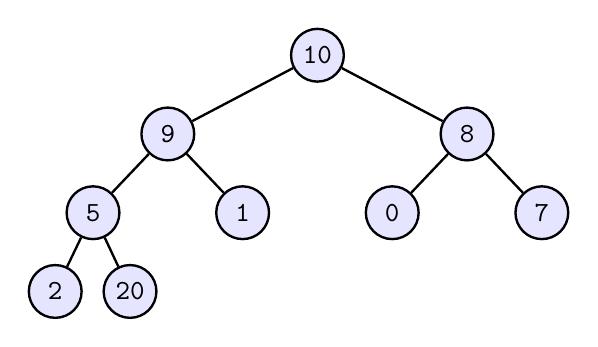
\begin{tikzpicture}

\fill[blue!10] (0.0, 0.0) circle (0.35);
\node [line width=0.03cm,black,minimum size=0.6699999999999999cm,draw,circle] at (0.0,0.0)(10){};\draw (0.0, 0.0) node[color=black] {\texttt{10}};
\fill[blue!10] (-1.9, -1.0) circle (0.35);
\node [line width=0.03cm,black,minimum size=0.6699999999999999cm,draw,circle] at (-1.9,-1.0)(9){};\draw (-1.9, -1.0) node[color=black] {\texttt{9}};
\fill[blue!10] (1.9, -1.0) circle (0.35);
\node [line width=0.03cm,black,minimum size=0.6699999999999999cm,draw,circle] at (1.9,-1.0)(8){};\draw (1.9, -1.0) node[color=black] {\texttt{8}};
\fill[blue!10] (-2.85, -2.0) circle (0.35);
\node [line width=0.03cm,black,minimum size=0.6699999999999999cm,draw,circle] at (-2.85,-2.0)(5){};\draw (-2.85, -2.0) node[color=black] {\texttt{5}};
\fill[blue!10] (-0.95, -2.0) circle (0.35);
\node [line width=0.03cm,black,minimum size=0.6699999999999999cm,draw,circle] at (-0.95,-2.0)(1){};\draw (-0.95, -2.0) node[color=black] {\texttt{1}};
\fill[blue!10] (0.95, -2.0) circle (0.35);
\node [line width=0.03cm,black,minimum size=0.6699999999999999cm,draw,circle] at (0.95,-2.0)(0){};\draw (0.95, -2.0) node[color=black] {\texttt{0}};
\fill[blue!10] (2.85, -2.0) circle (0.35);
\node [line width=0.03cm,black,minimum size=0.6699999999999999cm,draw,circle] at (2.85,-2.0)(7){};\draw (2.85, -2.0) node[color=black] {\texttt{7}};
\fill[blue!10] (-3.33, -3.0) circle (0.35);
\node [line width=0.03cm,black,minimum size=0.6699999999999999cm,draw,circle] at (-3.33,-3.0)(2){};\draw (-3.33, -3.0) node[color=black] {\texttt{2}};
\fill[blue!10] (-2.38, -3.0) circle (0.35);
\node [line width=0.03cm,black,minimum size=0.6699999999999999cm,draw,circle] at (-2.38,-3.0)(20){};\draw (-2.38, -3.0) node[color=black] {\texttt{20}};\draw[line width=0.03cm,black] (10) to  (9);
\draw[line width=0.03cm,black] (10) to  (8);
\draw[line width=0.03cm,black] (9) to  (5);
\draw[line width=0.03cm,black] (9) to  (1);
\draw[line width=0.03cm,black] (8) to  (0);
\draw[line width=0.03cm,black] (8) to  (7);
\draw[line width=0.03cm,black] (5) to  (2);
\draw[line width=0.03cm,black] (5) to  (20);
\end{tikzpicture}

\end{center}


So far we have
\[
a_0 = 1, \,\,\,\,\,
a_1 = 2, \,\,\,\,\,
a_2 = 4
\]
To simplify the problem, a line cannot go through a point of
intersection.
With three:
\begin{center}
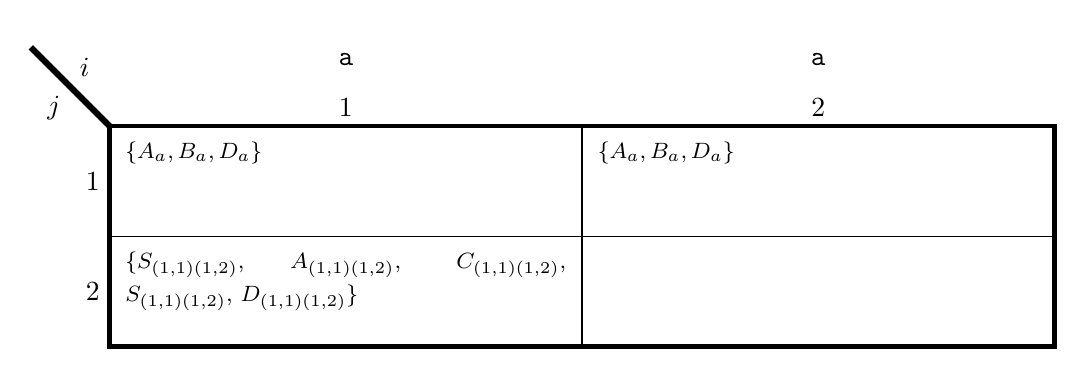
\begin{tikzpicture}

\draw (3.0, -0.7)
  node[draw, , , color=black,
       rounded corners=0cm, inner sep=0.2cm] {

\begin{minipage}[t][1.0cm]{5.6cm}
\mbox{}

\end{minipage}

};
\draw (3.0, -0.7) node[color=black,
 inner sep=0.2cm] {
 
\begin{minipage}[t][1.0cm]{5.6cm}
{\footnotesize $\{A_a,B_a,D_a\}$}
\end{minipage}

};
\draw (9.0, -0.7)
  node[draw, , , color=black,
       rounded corners=0cm, inner sep=0.2cm] {

\begin{minipage}[t][1.0cm]{5.6cm}
\mbox{}

\end{minipage}

};
\draw (9.0, -0.7) node[color=black,
 inner sep=0.2cm] {
 
\begin{minipage}[t][1.0cm]{5.6cm}
{\footnotesize $\{A_a,B_a,D_a\}$}
\end{minipage}

};
\draw (3.0, -2.0999999999999996)
  node[draw, , , color=black,
       rounded corners=0cm, inner sep=0.2cm] {

\begin{minipage}[t][1.0cm]{5.6cm}
\mbox{}

\end{minipage}

};
\draw (3.0, -2.0999999999999996) node[color=black,
 inner sep=0.2cm] {
 
\begin{minipage}[t][1.0cm]{5.6cm}
{\footnotesize $\{S_{(1,1)(1,2)},$ $A_{(1,1)(1,2)}$, $C_{(1,1)(1,2)}$, $S_{(1,1)(1,2)}$, $D_{(1,1)(1,2)} \}$}
\end{minipage}

};
\draw (9.0, -2.0999999999999996)
  node[draw, , , color=black,
       rounded corners=0cm, inner sep=0.2cm] {

\begin{minipage}[t][1.0cm]{5.6cm}
\mbox{}

\end{minipage}

};
\draw (9.0, -2.0999999999999996) node[color=black,
 inner sep=0.2cm] {
 
\begin{minipage}[t][1.0cm]{5.6cm}
{\footnotesize }
\end{minipage}

};\node[anchor=south] at (3.0,0.0) {1};\node[anchor=south] at (9.0,0.0) {2};\node[anchor=east] at (0,-0.7) {1};\node[anchor=east] at (0,-2.0999999999999996) {2};
\draw (6.0, -1.4)
  node[draw, line width=0.06cm, , color=black,
       rounded corners=0cm, inner sep=0cm] {

\begin{minipage}[t][2.8cm]{12.0cm}
\mbox{}

\end{minipage}

};\draw[line width=0.08cm,black] (0,0.0) to  (-1,1.0);
\node[anchor=north east] at (-0.5,0.5) {$j$};\node[anchor=south west] at (-0.5,0.5) {$i$};
\draw (3.0, 0.85)
  node[draw, line width=0.1cm, , color=white,
       rounded corners=0cm, inner sep=0cm] {

\begin{minipage}[t][0.7cm]{6.0cm}
\mbox{}

\end{minipage}

};\draw (3.0, 0.85) node[color=black] {{\texttt{a}}};
\draw (9.0, 0.85)
  node[draw, line width=0.1cm, , color=white,
       rounded corners=0cm, inner sep=0cm] {

\begin{minipage}[t][0.7cm]{6.0cm}
\mbox{}

\end{minipage}

};\draw (9.0, 0.85) node[color=black] {{\texttt{a}}};
\end{tikzpicture}

\end{center}

you get 7.
Note that the last line above, $L_3$, cuts through 3 regions,
and therefore adds 3 more
regions to the regions already obtained with the first two lines.
The next line will cut through 4 regions.
Come to think of it, $L_1$ (the first line) cuts through 1 region --
the uncut region,
$L_2$ (the second line) cuts through
2 regions.
In general line $L_n$ cuts through $n$ regions.
Now before $L_n$, therefore $a_{n-1}$ regions.
With $L_n$, the number of regions is $a_{n-1}$ and
$n$ regions are cut up by $L_n$. 
Therefore
\[
a_n = a_{n-1} + n
\]
for $n \geq 1$.


\newpage
\begin{ex}
What is $a_0$?
\qed
\end{ex}

\newpage
Let $a(x) = \sum_{n=0}^\infty a_n x^n$.
\begin{align*}
a(x) 
&= a_0 + \sum_{n=1}^\infty (a_{n-1} + n) x^n \\
&= a_0 + \sum_{n=1}^\infty a_{n-1} x^n + \sum_{n=0}^\infty n x^n \\
&= a_0 + x a(x) + \sum_{n=0}^\infty n x^n \\
\therefore\,\,\,\,\,\,
a(x) 
&= 
\frac{1 + x\frac{d}{dx} \sum_{n=0}^\infty x^n}{1 - x} \\
&=\frac{1 + x\frac{d}{dx} \frac{1}{1-x} }{1 - x} \\
&=\frac{1 + x \frac{1}{(1-x)^2} }{1 - x} \\
&=\frac{(1-x)^2 + x}{(1 - x)^2} \\
&=\frac{1 - x + x^2}{(1 - x)^3} \\
&=(1 - x + x^2) \sum_{n=0}^\infty \binom{3 + n - 1}{n} x^n \\
&=(1 - x + x^2) \sum_{n=0}^\infty \binom{n + 2}{2} x^n \\
&=
\sum_{n=0}^\infty \binom{n + 2}{2} x^n
- \sum_{n=0}^\infty \binom{n + 2}{2} x^{n+1}
+ \sum_{n=0}^\infty \binom{n + 2}{2} x^{n+2} \\
&=
\sum_{n=0}^\infty \binom{n + 2}{2} x^n
- \sum_{n=1}^\infty \binom{n + 1}{2} x^{n}
+ \sum_{n=2}^\infty \binom{n}{2} x^{n}
\end{align*}
Hence
\[
a_0 = 1, \,\,\,\,\,
a_1 = \binom{0 + 2}{2} + \binom{1 + 1}{2} = 2
\]
and for $n \geq 2$
\begin{align*}
a_n 
&= 
\binom{n + 2}{2} +
- \binom{n + 1}{2}
+ \binom{n}{2} \\
&= \frac{1}{2} 
((n+2)(n+1)
- (n+1)n
+ n(n-1)) \\
&= \frac{1}{2} 
(n^2 
+ n
+ 2)
\end{align*}
and note that this closed form 
can also be used for $a_0, a_1$.
Hence for $n \geq 0$
\begin{align*}
a_n 
= \frac{1}{2}
(n^2 
+ n
+ 2)
\end{align*}
or if you like
\begin{align*}
a_n 
= \frac{n(n+1)}{2} + 1
\end{align*}


\newpage
\begin{ex}
Instead of straight lines, what if we use lines bent at exactly one
point:
\begin{center}
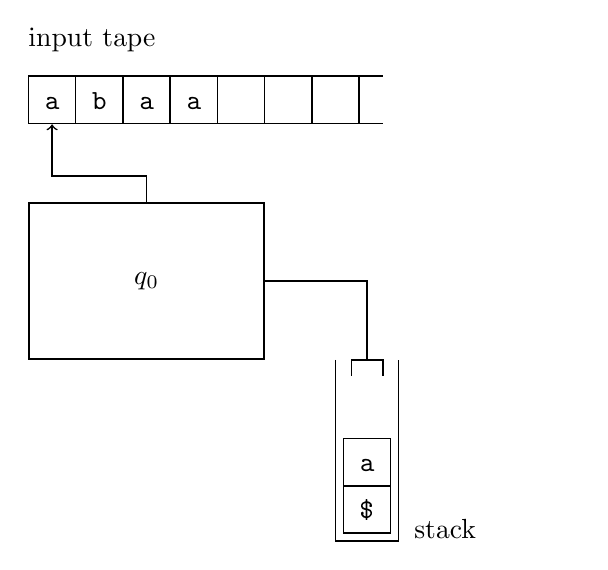
\begin{tikzpicture}

\draw (0.3, 0.3)
  node[draw, line width=0.02cm, , color=black,
       rounded corners=0cm, inner sep=0cm] {

\begin{minipage}[t][0.6cm]{0.6cm}
\mbox{}

\end{minipage}

};\draw (0.3, 0.3) node[color=black] {{\vphantom{a\$abaa\SPACE\SPACE\SPACE}\texttt{a}}};
\draw (0.8999999999999999, 0.3)
  node[draw, line width=0.02cm, , color=black,
       rounded corners=0cm, inner sep=0cm] {

\begin{minipage}[t][0.6cm]{0.6cm}
\mbox{}

\end{minipage}

};\draw (0.8999999999999999, 0.3) node[color=black] {{\vphantom{a\$abaa\SPACE\SPACE\SPACE}\texttt{b}}};
\draw (1.5, 0.3)
  node[draw, line width=0.02cm, , color=black,
       rounded corners=0cm, inner sep=0cm] {

\begin{minipage}[t][0.6cm]{0.6cm}
\mbox{}

\end{minipage}

};\draw (1.5, 0.3) node[color=black] {{\vphantom{a\$abaa\SPACE\SPACE\SPACE}\texttt{a}}};
\draw (2.0999999999999996, 0.3)
  node[draw, line width=0.02cm, , color=black,
       rounded corners=0cm, inner sep=0cm] {

\begin{minipage}[t][0.6cm]{0.6cm}
\mbox{}

\end{minipage}

};\draw (2.0999999999999996, 0.3) node[color=black] {{\vphantom{a\$abaa\SPACE\SPACE\SPACE}\texttt{a}}};
\draw (2.7, 0.3)
  node[draw, line width=0.02cm, , color=black,
       rounded corners=0cm, inner sep=0cm] {

\begin{minipage}[t][0.6cm]{0.6cm}
\mbox{}

\end{minipage}

};\draw (2.7, 0.3) node[color=black] {{\vphantom{a\$abaa\SPACE\SPACE\SPACE}\texttt{\SPACE}}};
\draw (3.3, 0.3)
  node[draw, line width=0.02cm, , color=black,
       rounded corners=0cm, inner sep=0cm] {

\begin{minipage}[t][0.6cm]{0.6cm}
\mbox{}

\end{minipage}

};\draw (3.3, 0.3) node[color=black] {{\vphantom{a\$abaa\SPACE\SPACE\SPACE}\texttt{\SPACE}}};
\draw (3.9000000000000004, 0.3)
  node[draw, line width=0.02cm, , color=black,
       rounded corners=0cm, inner sep=0cm] {

\begin{minipage}[t][0.6cm]{0.6cm}
\mbox{}

\end{minipage}

};\draw (3.9000000000000004, 0.3) node[color=black] {{\vphantom{a\$abaa\SPACE\SPACE\SPACE}\texttt{\SPACE}}};\draw[line width=0.02cm,black] (4.199999999999999,0.6) to  (4.5,0.6);
\draw[line width=0.02cm,black] (4.199999999999999,0.0) to  (4.5,0.0);

\draw (3.0, 1.1)
  node[draw=none, line width=0cm, , color=black,
       rounded corners=0cm, inner sep=0cm] {

\begin{minipage}[t][0.1cm]{6cm}
\mbox{}

\end{minipage}

};
\draw (3.0, 1.1) node[color=black,
 inner sep=0cm] {
 
\begin{minipage}[t][0.1cm]{6cm}
input tape
\end{minipage}

};
\draw (1.5, -2.0)
  node[draw, line width=0.02cm, , color=black,
       rounded corners=0cm, inner sep=0cm] {

\begin{minipage}[t][1.98cm]{2.98cm}
\mbox{}

\end{minipage}

};\draw (1.5, -2.0) node[color=black] {$q_0$};\draw[line width=0.02cm,black,->] (1.5,-1) to  (1.5,-0.67) to  (0.3,-0.67) to  (0.3,-0.01);

\draw (4.3, -4.3)
  node[draw, line width=0.02cm, , color=black,
       rounded corners=0cm, inner sep=0cm] {

\begin{minipage}[t][0.6cm]{0.6cm}
\mbox{}

\end{minipage}

};\draw (4.3, -4.3) node[color=black] {{\vphantom{a\$abaa\SPACE\SPACE\SPACE}\texttt{a}}};
\draw (4.3, -4.8999999999999995)
  node[draw, line width=0.02cm, , color=black,
       rounded corners=0cm, inner sep=0cm] {

\begin{minipage}[t][0.6cm]{0.6cm}
\mbox{}

\end{minipage}

};\draw (4.3, -4.8999999999999995) node[color=black] {{\vphantom{a\$abaa\SPACE\SPACE\SPACE}\texttt{\$}}};\draw[line width=0.02cm,black] (3.9,-3.0) to  (3.9,-5.3) to  (4.7,-5.3) to  (4.7,-3.0);

\draw (5.949999999999999, -5.1499999999999995)
  node[draw=none, line width=0cm, , color=black,
       rounded corners=0cm, inner sep=0cm] {

\begin{minipage}[t][0.1cm]{2.1cm}
\mbox{}

\end{minipage}

};
\draw (5.949999999999999, -5.1499999999999995) node[color=black,
 inner sep=0cm] {
 
\begin{minipage}[t][0.1cm]{2.1cm}
stack
\end{minipage}

};\draw[line width=0.02cm,black] (3,-2.0) to  (4.3,-2.0) to  (4.3,-3.0);
\draw[line width=0.02cm,black] (4.1,-3.2) to  (4.1,-3.0) to  (4.5,-3.0) to  (4.5,-3.2);
\end{tikzpicture}

\end{center}


For instance with two such lines
\begin{center}
\begin{tikzpicture}

\fill[white] (0.0, 0.0) circle (0.4);
\node [line width=0.03cm,black,minimum size=0.77cm,draw,circle] at (0.0,0.0)(1){};\draw (0.0, 0.0) node[color=black] {$p$};
\fill[white] (5.0, 0.0) circle (0.4);
\node [line width=0.03cm,black,minimum size=0.77cm,draw,circle] at (5.0,0.0)(2){};\draw (5.0, 0.0) node[color=black] {$q$};\draw[line width=0.03cm,black,->,>=triangle 60] (1) to node [above] {$\texttt{a}, \texttt{b} \rightarrow \texttt{c} $} (2);
\end{tikzpicture}

\end{center}


we can have 5 regions.
However this is not the maximum possible.
Show that it should be 7.
(HINT: See it? No?
Try to rotate one of the bent lines.)
Find a closed form for this problem.
\qed
\end{ex}

\newpage
\begin{ex}
  What if instead of lines or lines with one bend we have
  lines with 2 bends, i.e. something that looks like z and its reflection?
 What about lines with $k$ bends where $k$ is fixed?
  \qed
\end{ex}
  
\newpage
\begin{ex}
What if for the original problem we only count finite regions?
(i.e. we only count regions which are bounded on all sides by lines.)
\qed
\end{ex}

\newpage
\begin{ex}
What if instead of lines (or bent lines) we use
triangles?
\qed
\end{ex}


\newpage
\begin{ex}
What if instead of lines we use circles?
\qed
\end{ex}
